\subsection{Contract Field Test}
\label{sec:eval:cuad}

We use CUAD~\citep{ref_cuad} to test five fields: document name, agreement
date, effective date, expiration date or initial term, and governing law.
We select contracts with at most one distinct reference value per field
after whitespace cleanup and at most 40,000 source characters.
We keep the full source and check the positions of the labelled values.
Twenty official-training contracts form the development set.
All 56 official-test contracts that meet the rules form the test set.

We compare initial extraction, Simple repair, indexed repair, and indexed
fresh extraction. Both repair methods receive the same initial graph.
The indexed methods add field-line windows to the full source.
All settings share the Gemma model, field meanings, and a 4,000-token output
limit. Before collection, we set the code to handle JSON fences and assign
document IDs. We keep the prompts and selection rules fixed after one
development round.

\begin{table}[t]
\centering
\caption{Contract results on 56 documents. F1 checks exact text after whitespace cleanup. Lost counts correct input facts removed. The input row gives the initial graph cost; repair rows give the repair-call cost.}
\label{tab:cuad}
\small
\begin{tabular}{lrrrr}
\toprule
Output & F1 (\%) & Lost & New incorrect & Requests \\
\midrule
Initial extraction & 46.76 & 0 & 0 & 59 \\
Simple repair & 43.35 & 7 & 2 & 71 \\
Indexed repair & 44.84 & 5 & 12 & 69 \\
Indexed re-extraction & 44.12 & 8 & 32 & 71 \\
\bottomrule
\end{tabular}
\end{table}

Indexed repair reaches 44.84\% F1, compared with 46.76\% for the input,
a 1.92-point drop. It removes five correct input facts and adds twelve
facts that differ from the reference. Simple repair also scores below
the input.

Indexed repair leads indexed fresh extraction by 0.72 F1 points
(95\% paired CI: [-4.80,6.48]; sign-flip $p=0.810$).
The test gives 224 outputs from 270 requests, including retries.
Failed outputs are scored as empty graphs.
The score checks copied text against CUAD labels after whitespace cleanup.

\begin{figure}[t]
\centering
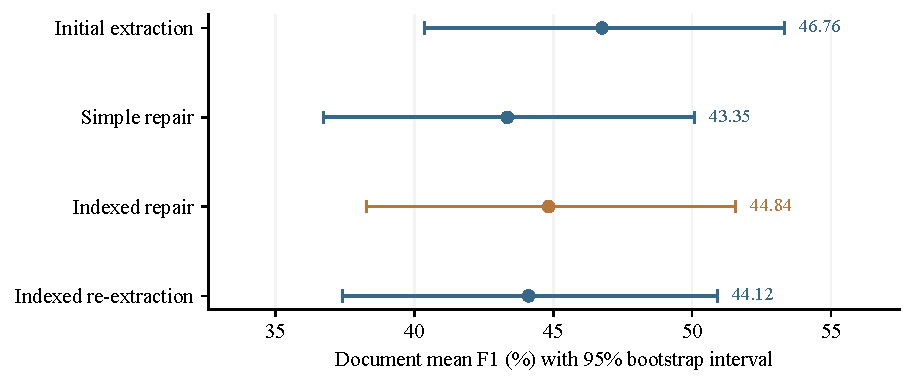
\includegraphics[width=0.88\textwidth]{figure/experiments/cuad_contracts.pdf}
\caption{Contract scores. Points show mean document F1. Bars show 95\% CIs for each method. The text gives the paired repair--extraction CI.}
\label{fig:cuad}
\end{figure}
